\section{Experiments}\label{sec:experiments}

\subsection{Experiment setup}
The experiments were performed doing one versus all classification. The data for each expression is divided into a training and a validation set and an SVM
classifier is calculated based on the training set. The accuracy of the classifiers is then measured on the validation set. It was ensured that images of the same
person are not present in both the training and validation set. The fraction of the data used for the validation set is a configurable parameter, for the
following experiments 75\% of the data was used for the training set and 25\% for the validiation set.

\subsection{Validation of Manually Extracted Patches}\label{sec:experiments:manual}
Tables \ref{table:left_eye}, \ref{table:right_eye}, \ref{table:between_eyes} and \ref{table:mouth} show the ratios of correct detections for eight facial expressions for each region, for classifiers trained with the original patch size of 96x96 and also rescaled to 32x32 and 64x64 pixels. Shrinking the images on the one hand results in fewer hog features which is likely to reduce the effect of overfitting, on the other hand some visual information may be lost. The table entries represent the fraction of the images of the corresponding expression that were correctly classified, in the 0 to 1 range.


%\subsection{Results}

\begin{table}

    \begin{subtable}[b]{3in}
    \centering
    \begin{tabular}{| c | c | c | c |}
    \hline
    Expression & 32 x 32 &  64 x 64  & 96 x 96  \\
    \hline
    Angry & 0.5865 & 0.6786 & 0.7068 \\
    Contempt & 0.6596 &	0.5745 & 0.5532 \\
    Disgust	& 0.7629 &	0.7629 &	0.7716 \\
    Fear &	0.6155 & 0.6315 & 0.6394 \\
    Happy &	0.6074 & 0.6605 & 0.6529 \\
    Neutral & 0.6851 &	0.6996 & 0.7093 \\
    Sadness & 0.5207 & 0.5041 &	0.5021 \\
    Surprise & 0.7652 &	0.7683 & 0.7561 \\
    \hline
    \end{tabular}
    \caption{Left eye patches}
    \label{table:left_eye}
    \end{subtable}
\quad


    \begin{subtable}[b]{3in}
    \centering
    \begin{tabular}{| c | c | c | c |}
    \hline
    Expression & 32 x 32 &  64 x 64  & 96 x 96  \\
    \hline
    Angry    & 0.5733 & 0.6466 & 0.6654 \\
    Contempt & 0.5638 & 0.5106 & 0.6170 \\
    Disgust	 & 0.7263 & 0.7414 & 0.7155 \\
    Fear	 & 0.6474 & 0.6076 & 0.6096 \\
    Happy	 & 0.6367 & 0.6334 & 0.6833 \\
    Neutral  & 0.7099 & 0.7272 & 0.7562 \\
    Sadness  & 0.5000 & 0.5207 & 0.5456 \\
    Surprise & 0.7896 & 0.8171 & 0.8079 \\
    \hline
    \end{tabular}
    \caption{Right eye patches}
    \label{table:right_eye}
    \end{subtable}
\quad


    \begin{subtable}[b]{3in}
    \centering
    \begin{tabular}{| c | c | c | c |}
    \hline
    Expression & 32 x 32 &  64 x 64  & 96 x 96  \\
    \hline
    Angry & 0.7971 & 0.812 & 0.7857 \\
    Contempt & 0.4468 & 0.4574 & 0.4681 \\
    Disgust & 0.6983 & 0.7155 & 0.7306 \\
    Fear & 0.7071 & 0.7649 & 0.7351 \\
    Happy & 0.8503 & 0.8503 & 0.8329 \\
    Neutral & 0.7438 & 0.7845 & 0.7921 \\
    Sadness & 0.7324 & 0.7697 & 0.7635 \\
    Surprise & 0.7317 & 0.7485 & 0.7165 \\
    \hline
    \end{tabular}
    \caption{Right eye patches}
    \label{table:between_eyes}
    \end{subtable}
\quad


    \begin{subtable}[b]{3in}
    \centering
    \begin{tabular}{| c | c | c | c |}
    \hline
    Expression & 32 x 32 &  64 x 64  & 96 x 96  \\
    \hline
    Angry	&	0.7782	&	0.8064	&	0.7970	\\
    Contempt	&	0.6277	&	0.6598	& 0.6702 \\
    Disgust	&	0.6918	&	0.7953	&	0.8039	\\
    Fear	&	0.7510	&	0.8287	&	0.8307	\\
    Happy	&	0.8959	&	0.9121	&	0.9154	\\
    Neutral	&	0.7974	&	0.8577	&	0.8501	\\
    Sadness	&	0.8589	&	0.8651	&	0.8693	\\
    \hline
    \end{tabular}
    \caption{Mouth patches}
    \label{table:mouth}
    \end{subtable}

\label{table:results of patches}
\caption[Ratios of correct detections for eight facial expressions]{Ratios of correct detections for eight facial expressions. Table \ref{table:left_eye}, Table \ref{table:right_eye}, Table \ref{table:between_eyes} and Table \ref{table:mouth} shows the result of all left-eye patches, all right-eye patches, patches of the part between eyes and all mouth patches respectively. The results of four kind of patches were all based on the sizes of 32x32 pixels, 64x64 pixels and 96x96 pixels.}
\end{table}

\subsection{Classification of Entire Facial Images}
We also experimented with training SVM classifiers considering the entire facial area as a single patch. First the bounding box of the face was detected
for each image using the Viola-Jones algorithm, then rescaled to a uniform size. % TODO: Add Reference.
The rest of the procedure was identical to the preceding experiment. The results can be found in Table \ref{table:entire_images}.

\begin{table}
\begin{tabular}{| c | c | c | c |}
\hline
Expression & 32 x 32 &  64 x 64  & 96 x 96  \\

\hline
Angry	 & 0.6165 & 0.6316 & 0.6297	\\
Contempt & 0.4894 & 0.5000 & 0.4043	\\
Disgust	 & 0.7109 & 0.8793 & 0.9367	\\
Fear	 & 0.3540 & 0.6574 & 0.6420	\\
Happy	 & 0.8080 & 0.9317 & 0.9360	\\
Neutral	 & 0.7203 & 0.8260 & 0.8225	\\
Sadness	 & 0.5996 & 0.5830 & 0.6432	\\
Surprise & 0.8765 & 0.9405 & 0.9665	\\

\hline
\end{tabular}
\caption{Classifying the whole image}
\label{table:entire_images}
\end{table}


\subsection{Classification of Expression Development}
After training SVM classifier, we needed to know whether the classifier is able to predict and classify the images of a complete time series, where the emotional expression develops from neutral to the particular peak expression. We picked out all aligned patches (the part between eyes, left eye, right eye and mouth) from one subject with complete time series for each emotion. An example of extracted mouth patches from a happy person can be seen in figure \ref{fig:timeseriesHappy}. As shown in the previous experiments in section \ref{sec:experiments:manual}, rescaling has no great influence on the results, so all patches in this experiment were of the size of 96x96 pixels. We listed the best classifications, the prediction provided of mouth and right-eye patches, in the table \ref{table:predict_series}. The results show, which images are still regarded as neutral and which image marks the point towards the concrete emotional expression. They also show, that the images, where the expression changes, can not always be clearly classified, while the mouth patches still provide more stable and correct results than the eye patches.

\begin{figure}%[H]
	\centering
	\begin{subfigure}[b]{0.15\textwidth}
		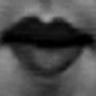
\includegraphics[width=\textwidth]{./img/timeseriesHappy/S026_006_00000001_conew1.png}
		\caption{}
		\label{fig:timeseriesHappy:a}
	\end{subfigure}
	%\hspace{\fill}
	\begin{subfigure}[b]{0.15\textwidth}
		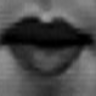
\includegraphics[width=\textwidth]{./img/timeseriesHappy/S026_006_00000002_conew1.png}
	  \caption{}
		\label{fig:timeseriesHappy:b}
	\end{subfigure}
	%\hspace{\fill}
	\begin{subfigure}[b]{0.15\textwidth}
		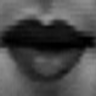
\includegraphics[width=\textwidth]{./img/timeseriesHappy/S026_006_00000003_conew1.png}
		\caption{}
		\label{fig:timeseriesHappy:c}
	\end{subfigure}
	%\hspace{\fill}
	\begin{subfigure}[b]{0.15\textwidth}
		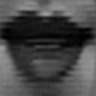
\includegraphics[width=\textwidth]{./img/timeseriesHappy/S026_006_00000004.png}
		\caption{}
		\label{fig:timeseriesHappy:d}
	\end{subfigure}
	%\hspace{\fill}
	\begin{subfigure}[b]{0.15\textwidth}
		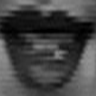
\includegraphics[width=\textwidth]{./img/timeseriesHappy/S026_006_00000005.png}
		\caption{}
		\label{fig:timeseriesHappy:e}
	\end{subfigure}
	%\hspace{\fill}
	\begin{subfigure}[b]{0.15\textwidth}
		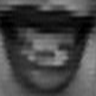
\includegraphics[width=\textwidth]{./img/timeseriesHappy/S026_006_00000006.png}
		\caption{}
		\label{fig:timeseriesHappy:f}
	\end{subfigure}
	%\hspace{\fill}
	\begin{subfigure}[b]{0.15\textwidth}
		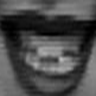
\includegraphics[width=\textwidth]{./img/timeseriesHappy/S026_006_00000007.png}
		\caption{}
		\label{fig:timeseriesHappy:g}
	\end{subfigure}
	%\hspace{\fill}
	\begin{subfigure}[b]{0.15\textwidth}
		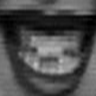
\includegraphics[width=\textwidth]{./img/timeseriesHappy/S026_006_00000008.png}
		\caption{}
		\label{fig:timeseriesHappy:h}
	\end{subfigure}
	%\hspace{\fill}
	\begin{subfigure}[b]{0.15\textwidth}
		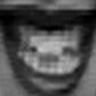
\includegraphics[width=\textwidth]{./img/timeseriesHappy/S026_006_00000009.png}
		\caption{}
		\label{fig:timeseriesHappy:i}
	\end{subfigure}
	%\hspace{\fill}
	\begin{subfigure}[b]{0.15\textwidth}
		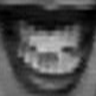
\includegraphics[width=\textwidth]{./img/timeseriesHappy/S026_006_00000010.png}
		\caption{}
		\label{fig:timeseriesHappy:j}
	\end{subfigure}
	%\hspace{\fill}
	\begin{subfigure}[b]{0.15\textwidth}
		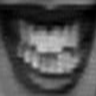
\includegraphics[width=\textwidth]{./img/timeseriesHappy/S026_006_00000011.png}
		\caption{}
		\label{fig:timeseriesHappy:k}
	\end{subfigure}
	%\hspace{\fill}
	\begin{subfigure}[b]{0.15\textwidth}
		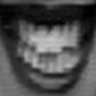
\includegraphics[width=\textwidth]{./img/timeseriesHappy/S026_006_00000012.png}
		\caption{}
		\label{fig:timeseriesHappy:l}
	\end{subfigure}
	%\hspace{\fill}
	\begin{subfigure}[b]{0.15\textwidth}
		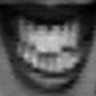
\includegraphics[width=\textwidth]{./img/timeseriesHappy/S026_006_00000013.png}
		\caption{}
		\label{fig:timeseriesHappy:m}
	\end{subfigure}
	\caption[Complete time series of happy mouth patches]{Extracted mouth patch of size 96x96 pixels showing the development of
	the facial expression of happiness from neutral to maximal happy expression.
	Patches \ref{fig:timeseriesHappy:a} to \ref{fig:timeseriesHappy:c} have been
	categorized for training as neutral, patches \ref{fig:timeseriesHappy:d} to
	\ref{fig:timeseriesHappy:g} have been excluded from training and patches
	\ref{fig:timeseriesHappy:e} to \ref{fig:timeseriesHappy:m} have been used as
	positive samples for training happy expressions. Classification identified
	\ref{fig:timeseriesHappy:a} to \ref{fig:timeseriesHappy:c} correctly as
	neutral, \ref{fig:timeseriesHappy:d} was identified as disgust and
	\ref{fig:timeseriesHappy:e} to \ref{fig:timeseriesHappy:m} were classified as
	happy expressions according to table \ref{table:predict_series}.}
	\label{fig:timeseriesHappy}
\end{figure}


\subsection{Classification of Unaligned Patches}
Moreover, we also experimented with some patches from several subjects which were not aligned with training data. These pathes were all from intense expressions of our dataset. The predicted patches were of size 96x96 pixels because rescaling has no effect as mentioned. We experimented with four kind of patches respectively from one emotion and observed how much outputs would match. Table \ref{table:predict_unaliged_surprise} and Table \ref{table:predict_unaliged_fear} listed the results of patches from 15 subjects in the surprise and fear emotions. The results will indicate the effect of alignment of patches.

\begin{table*}
\centering

    \begin{subtable}{4.7in}
    %\centering
    \begin{tabular}{|*{15}{p{1.34cm}<{\centering}|}|}
    \hline
    Time & Angry &  Disgust  & Fear & Happy & Sadness & Surprise  \\
    \hline
    1 & neutral & neutral & neutral & neutral & neutral & neutral \\
    2 & neutral & neutral & neutral & neutral & neutral & neutral \\
    3 & neutral & neutral & neutral & neutral & neutral & neutral \\
    4 & neutral & neutral & neutral & disgust & neutral & neutral \\
    5 & neutral & neutral &neutral & happy & neutral & neutral \\
    6 & neutral & neutral & disgust & happy & neutral & disgust \\
    7 & neutral & disgust & fear & happy & neutral & surprise \\
    8 & neutral & disgust & fear & happy & neutral & surprise \\
    9 & neutral & disgust & fear & happy & sadness & surprise \\
    10 & contempt & disgust & fear & happy & sadness & surprise \\
    11 & neutral & disgust & fear & happy & sadness & surprise \\
    12 & contempt & disgust & fear & happy & sadness & surprise \\
    13 & angry & disgust & fear & happy & sadness & surprise \\
    14 & angry & disgust & fear & happy & sadness & surprise \\
    15 & angry & disgust & fear & happy & sadness & surprise\\
     \hline
    \end{tabular}
    \caption{Aligned mouth patches}
    \label{table:predict_series:mouth}
    \end{subtable}

    \begin{subtable}{4.7in}
    %\centering
    \begin{tabular}{|*{15}{p{1.34cm}<{\centering}|}|}
    \hline
    Time & Angry &  Disgust  & Fear & Happy & Sadness & Surprise  \\
    \hline
    1 & disgust & neutral & neutral & neutral & neutral & neutral \\
    2 & neutral & disgust & neutral & neutral & neutral & neutral \\
    3 & neutral & neutral & neutral & neutral & neutral & neutral \\
    4 & disgust & neutral & neutral & contempt & neutral & neutral \\
    5 & neutral & contempt & neutral & contempt & neutral & neutral	\\
    6 & happy & contempt & neutral & contempt & contempt & neutral \\
    7 & contempt & disgust & neutral & happy & contempt & neutral \\
    8 & neutral & disgust & contempt & happy & neutral & neutral \\
    9 & contempt & disgust & happy & happy & sadness & surprise \\
    10 & contempt & disgust & contempt & happy & sadness & surprise	\\
    11 & contempt & disgust & contempt & happy & sadness & surprise \\
    12 & neutral & disgust & neutral & happy & sadness & surprise \\
    13 & contempt & disgust & contempt & happy & sadness & surprise \\
    14 & contempt & disgust & neutral & happy & sadness & surprise \\
    15 & neutral & disgust & neutral & happy & sadness & surprise\\

    \hline
    \end{tabular}
    \caption{Aligned right-eye patches}
    \label{table:predict_series:righteye}
    \end{subtable}

\caption[Results of prediction of aligned patches]{Results of prediction of aligned mouth and right-eye patches with time series from all images of one subject. That means each kind of patches was ordered from neutral to intense one. All predicted patches were of size 96x96 pixels. }
\label{table:predict_series}
\end{table*}


\begin{table}

    \begin{subtable}{3in}
    \newcommand{\tabincell}[2]{\begin{tabular}{@{}#1@{}}#2\end{tabular}}
    \begin{tabular}{|*{1}{p{0.3cm}<{\centering}|} c | c | c | c |}
    \hline
      & Mouth & Left-eye  & Right-eye & \tabincell{c}{Part \\ between\\ eyes}  \\
    \hline
    1 & sadness & disgust & surprise & fear \\
    2 & sadness & fear & disgust & fear \\
    3 & neutral & surprise & happy & disgust \\
    4 & neutral & disgust & happy & surprise \\
    5 & disgust & fear & disgust & fear \\
    6 & surprise & fear & sadness & disgust \\
    7 & surprise & surprise & sadness & disgust \\
    8 & disgust & sadness & disgust & fear \\
    9 & surprise & angry & surprise & surprise \\
    10 & fear & surprise & disgust & surprise \\
    11 & surprise & angry & sadness & fear \\
    12 & surprise & angry & disgust & disgust \\
    13 & fear & surprise & disgust & disgust \\
    14 & surprise & fear & surprise & disgust \\
    15 & surprise & surprise & fear & fear \\
    \hline
    \end{tabular}
    \caption{Unaligned patches from surprise emotion}
    \label{table:predict_unaliged_surprise}
        \end{subtable}
\qquad

    \begin{subtable}{3in}
    \newcommand{\tabincell}[2]{\begin{tabular}{@{}#1@{}}#2\end{tabular}}
    \begin{tabular}{|*{1}{p{0.3cm}<{\centering}|} c | c | c | c |}
    \hline
      & Mouth &  Left-eye  & Right-eye & \tabincell{c}{Part \\ between\\ eyes} \\
    \hline
    1 & happy & fear & fear & disgust \\
    2 & happy & disgust & fear & fear \\
    3 & contempt & surprise & contempt & fear \\
    4 & contempt & disgust & contempt & disgust \\
    5 & fear & disgust & disgust & fear \\
    6 & fear & fear & sadness & angry \\
    7 & disgust & sadness & sadness & surprise \\
    8 & fear & disgust & disgust & angry \\
    9 & fear & disgust & disgust & fear \\
    10 & fear & surprise & disgust & disgust \\
    11 & fear & surprise & surprise & fear \\
    12 & contempt & fear & disgust & fear \\
    13 & fear & disgust & disgust & surprise \\
    14 & contempt & disgust & fear & disgust \\
    15 & happy & fear & fear & disgust \\
    \hline
    \end{tabular}
    \caption{Unaligned patches from fear emotion}
    \label{table:predict_unaliged_fear}
    \end{subtable}

    \caption[Results of prediction of unaligned patches]{Results of prediction of unaligned patches with size of 96x96 from 15 subjects in the dataset. Table \ref{table:predict_unaliged_surprise} and Table \ref{table:predict_unaliged_fear} shows the outputs of four kind of patches in the surprise and fear emotions}
    \label{table:predict_unaliged_image}
\end{table}
